%% LaTeX2e class for student theses
%% sections/content.tex
%% 
%% Karlsruhe Institute of Technology
%% Institute for Program Structures and Data Organization
%% Chair for Software Design and Quality (SDQ)
%%
%% Dr.-Ing. Erik Burger
%% burger@kit.edu
%%
%% Version 1.3, 2016-12-29

\chapter{Introduction}
\label{ch:Introduction}

During the introduction we will \textit{motivate} (\autoref{sec:Introduction:motivation}) for the topic at hand and introduce the \textit{problems} (\autoref{sec:Introduction:problems}) arising from it. Further, we will introduce the \textit{goal and research questions} (\autoref{sec:Introduction:goals}) handled in this thesis. Finally, we will give a short \textit{outline} (\autoref{sec:Introduction:outline}) about the remainder chapters.


\section{Motivation}
\label{sec:Introduction:motivation}

Over the last years, cloud computing has become more and more popular. This is a result of its business advantages, the continuing simplification of its usage and the abundance of own data centres. Netflix, for example, closed all its owned data centre in 2015 and moved completely to Amazons AWS\cite{DavidChernicoff.2015}. This trend results in the expected revenue of about 200 Billion \$ in 2016\cite{statista.com.2016}. The high degree of elasticity, automation, self-service, flexibility in payment and, as a result, lower cost are only some of the many advantageous points of cloud computing.\cite{Binz.2014}

However, many – especially European - companies fear dependencies, loss of data control, industrial espionage or privacy law violations. Precautionary measures like encryption or data splitting - among data centres - is not enough to prevent a public relations disaster, due to complex EU Data Protective Regulations\cite{personaldata.2011} or the US HIPAA act\cite{OfficeforCivilRights.20130726}. To tell the whole truth, the complexity, the hidden usage of services and the therefore resulting unawareness of many EU citizens (and law enforcement institutes) makes it very unlikely for current law violators to face any consequences. Nevertheless, citizens start to be more aware and the law enforcement point of attention tends to change quickly, like the Max Schrems' "Facebook Process" showed \cite{JuliaBahr.20150923}. Further, in 2018 the "reform of EU data protection rules" will come into force, which states severe punishments for privacy violations\cite{personaldata.2011}. As a result, entrepreneurs, companies and institutions need to be more aware of privacy compliance to prevent major monetary and reputation losses. 

The \textit{EU General Data Protection Regulations} sets the legal boundaries for European companies. It defines multiple regulations about data handling, data trading, personal advertising and more. One rule sets the boundaries for personal data processing and saving. It states, for example, that the processing of personal data is only allowed in data centres inside the EU or certain certified countries with equivalent privacy laws. As a result, software systems require a pre-deployment law compliance checking, considering especially the hosts geo-locations. The problem comes to a head with the ease of migration of whole cloud services during runtime with next to no downtime. With this in mind a potential privacy violation could occur even though the initial deployment was law compliant. This requires a non-stop observation of the applications geo-location and automatic, law compliant redeployment onto other cloud providers.


\section{Problems}
\label{sec:Introduction:problems}

To create such a privacy aware system adaptor, a couple of non-trivial problems need to be solved. The major ones will be outlined shortly, categorized after the MAPE-K feedback loop \cite{Dar.2012}.

Initially, we need to \textit{acquire} the geo-location information of a cloud server. This is the fundamental task to be able to determine whether a system is compliant to the \textit{EU General Data Protection Regulations} or the \textit{HIPAA} act. Further, we need to \textit{store} this information adequately in the available information sources. In our case that is the \textit{Palladio Component Model} (PCM), an architecture description language. However, the PCM is not designed to store geo-information of any kind.

After the acquisition of the geo-location information, we need to determine, whether the observed system is in a privacy compliant state. We refer to this task as \textit{privacy analysis}. The major obstacles for the privacy analysis are the limited information about the system and the complicated legal regulations. So, the problem is to gain a meaningful result, without significantly extending the information sources or increasing the PCM complexity.

During the planning phase, a privacy \textit{alternative system deployment} needs to be calculated. While automated performance optimization was achieved in the past, the privacy compliance has never been considered during this task. Depending on the parameters, alternative generation and evaluators this is a considerable problem and optimization task.

To regain a privacy compliant system state, the system needs to be modified towards the generated alternative. For this task, the \textit{system adaptation} steps need to be calculated and ordered. The migration of a live system usually inflicts man dependencies and ripple effects that have to be considered before executing these steps.

We provided a rough overview of the problems at hand. Further details and the according solution will be explained in the according chapters of this thesis.
%\begin{itemize}
%	\setlength\itemsep{0em}
%	\item \textbf{Monitoring}\newline
%	Acquiring and transforming geo-location information onto an architecture description language
%	\item \textbf{Analysing}\newline
%	Privacy compliance analysis on a software architecture basis
%	\item \textbf{Planning}\newline
%	Computation of constraint and privacy compliant redeployments
%	\item \textbf{Executing}\newline
%	Technology independent, dynamic adaptation routine computation and execution
%\end{itemize}

%Transformation for geo-location into ADL
%Privacy analysis on architecture lvl
%Privacy compliant system deployment calculation
%System adaptation calculation
%System adaptation execution

%simple & efficient privacy concept for component based architecture
%what information are required?
%
%
%automatic migration with evaluation


\section{Goals and Research Questions}
\label{sec:Introduction:goals}

This thesis' goal is to contribute and outline a piece of software, that ensures continues privacy compliance, modelled after the MAPE-K feedback loop. Connected to this goal, a number of important research questions arise:

\begin{itemize}
	\setlength\itemsep{0em}
	\item \textbf{Monitoring} %How can information, required for privacy violation detection, be monitored? How can we transform this information onto our architecture model?
	\begin{itemize}
		\setlength\itemsep{0em}
		\item \textbf{RQ-M1}: How can the required information be monitored and transformed into the architectural description language?
		\item \textbf{RQ-M2}: How accurate is the monitoring and transformation?
		\item \textbf{RQ-M3}: How good does the monitoring and transformation scale?
	\end{itemize}
		\item \textbf{Analysing} %How to analyse the model for privacy violation detection? And how good does this analysis scale?
	\begin{itemize}
		\setlength\itemsep{0em}
		\item \textbf{RQ-A1}: How can we detect privacy violations on a architectural level?
		\item \textbf{RQ-A2}: Are there scenarios that can not be detect?
		\item \textbf{RQ-A3}: How good does the privacy analysis scale with the system size?
	\end{itemize}

	\item \textbf{Planning} %How can the runtime model and analysis results be used to reacquire policy compliance?
	\begin{itemize}
		\setlength\itemsep{0em}
		\item \textbf{RQ-P1}: How can we generate an alternative, privacy compliant deployment?
		\item \textbf{RQ-P2}: How accurate is the alternative generation?
	\end{itemize}

	\item \textbf{Executing} %How can the plan automatically be executed and policy compliance established? How much human interaction is necessary?
	\begin{itemize}
		\setlength\itemsep{0em}
		\item \textbf{RQ-E1}: How can we calculate an automated system adaptation sequence?
		\item \textbf{RQ-E2}: How good does the adaptation calculation work?
		\item \textbf{RQ-E3}: How good does the adaptation scale with the system size and the potential modifications?
	\end{itemize}
\end{itemize}


\section{Outline}
\label{sec:Introduction:outline}

The remainder of this thesis is structured as follows: The thesis continues by introducing the foundations (\autoref{ch:Foundations}) and the related work (\autoref{ch:RelatedWork}) of this thesis. The main part starts with the privacy concept (\autoref{ch:PrivacyConcept}), leading into the system overview (\autoref{ch:Overview}), followed by the big conceptual work packages: Palladio extension (\autoref{ch:pcmExtension}), iObserve extension (\autoref{ch:iObserve}), privacy analysis (\autoref{ch:PrivacyAnalysis}), PerOpteryx extension (\autoref{ch:PerOpt}) and the system adaptation (\autoref{ch:SysAdap}). The thesis closes with the evaluation (\autoref{ch:Evaluation}) and finally the conclusion (\autoref{ch:Conclusion}).



%%%%%%%%%%%%%%%%%%%%%%%%%%%%%%%%%%%%%%%%%%%%%%%%%%%%%%%%%%%%%%%%%%%%%%
\chapter{Foundations}
\label{ch:Foundations}

In this chapter we will introduce applications and principles on which this thesis is based on. This introduction aims for a general understanding. We would like to point out that some topics may be discussed in more detail in the corresponding section.

\section{MAPE-K loop}
\label{sec:Foundations:mape}

MAPE-K or MAPE was first introduced by IBM for automatic computing and later discussed in the context of self-adaptive systems. A MAPE system is usually a stand alone application, which is specially build for optimizing and adapting a monitored system. MAPE-K is an acronym, consisting of the first letters of the loops stages: Monitor, Analyse, Plan, Execute and Knowledgebase. These stages are sequentially ordered in a pipeline structure, each one has a well defined task \cite{Dar.2012}:

\begin{itemize}
	\setlength\itemsep{0em}
	\item \textbf{Monitor}: Collects, aggregates, filters and correlates information about a monitored system.
	\item \textbf{Analyse}: Performs (complex) data analysis and reasoning on the monitored data. The analysis is often supported by data from the knowledgebase. If changes are required, a change request is passed to the plan function.
	\item \textbf{Plan}: Determines what kind of changes are required and develops a transformation which adapts the monitored system towards the desired state.
	\item \textbf{Execute}: Executes the transformation calculated during the planning phase.
	\item \textbf{Knowledgebase}: Additional or advanced information that are shared among all stages.
\end{itemize}

The monitored system runs independently from the MAPE application. However, the desired monitoring information are usually explicitly provided via specially designed APIs, intefaces or probes \cite{Dar.2012}.


\section{Palladio Component Model}
\label{sec:Foundations:pcm}

The Palladio Component Model (short PCM) is an Architecture Description Language (ADL) for component based software, originally designed to enable software architects to run pre-implementation performance analysis. The Palladio Simulator reports on "performance bottlenecks, scalability issues, reliability threats, and allows for a subsequent optimisation." The PCM is composed of several sub-models which depend on another. Each model represents a certain aspect of a component based software:

\begin{itemize}
	\setlength\itemsep{0em}
	\item \textbf{Repository Model}: Defines Components with required and provided interfaces. Interfaces include function signatures. 
	\item \textbf{System Model}: Defines the complete software system, by connecting components defined in the repository model.
	\item \textbf{Usage Model}: Defines process workload, based on the systems interfaces.
	\item \textbf{Resource Environment Model}: Defines available host environments with its provided performance.
	\item \textbf{Allocation Model}: Defines the deployment of system components onto the provided hosts.
\end{itemize}

The separation of concern enables the system architect to manage the complexity of even bigger software systems and still gain meaningful results from the performance simulation.

Since its initial release, the Palladio Component Model was adapted and used in several research fields alongside the performance prediction, like automated Dataflow Analysis and Application Monitoring. Due to its explicit representation of the software architecture and flexible component-host-mapping it is perfectly suited to model distributed cloud systems. Although, PCM was not designed to be used as a runtime model, it has proven to be suited for this task due to its versatile model elements \cite{Becker.2009}.

\section{Kieker}
\label{sec:Foundations:Kieker}

Kieker is a software system monitoring application with the goal of retrieving runtime information for performance evaluation, (self-)adaptation control and many other tasks. Kieker gains these information from the designated software by instrumenting the system with probes during pre-compilation. Each probe has designated purpose and gathers data accordingly, for example hardware utilization, stack trace or host geo-location. Kieker uses event-based probes, as well as periodic-based (heart-beat) probes \cite{kieker.web}.


\section{iObserve}
\label{sec:Foundations:iobserve}

iObserve is a system optimization tool after the MAPE feedback loop. The two primary goals are an automated system adaptation and an \textit{operator-in-the-loop} system evolution (see \autoref{fig:intro:iObserve}).

For the initial MAPE step, monitoring, iObserve uses Kieker. The gathered information are transformed onto a Palladio Component Model. Due to the live characteristic this PCM model is called a runtime model. Further, iObserve is designed to support distributed cloud systems. Key features of the transformation are the processing stack trace information for usage model updates, so more precise performance simulations are possible. Further the processing of deployment and un-deployment events, as well as hardware utilization  measurements.

\begin{figure}[h]
	\centering
	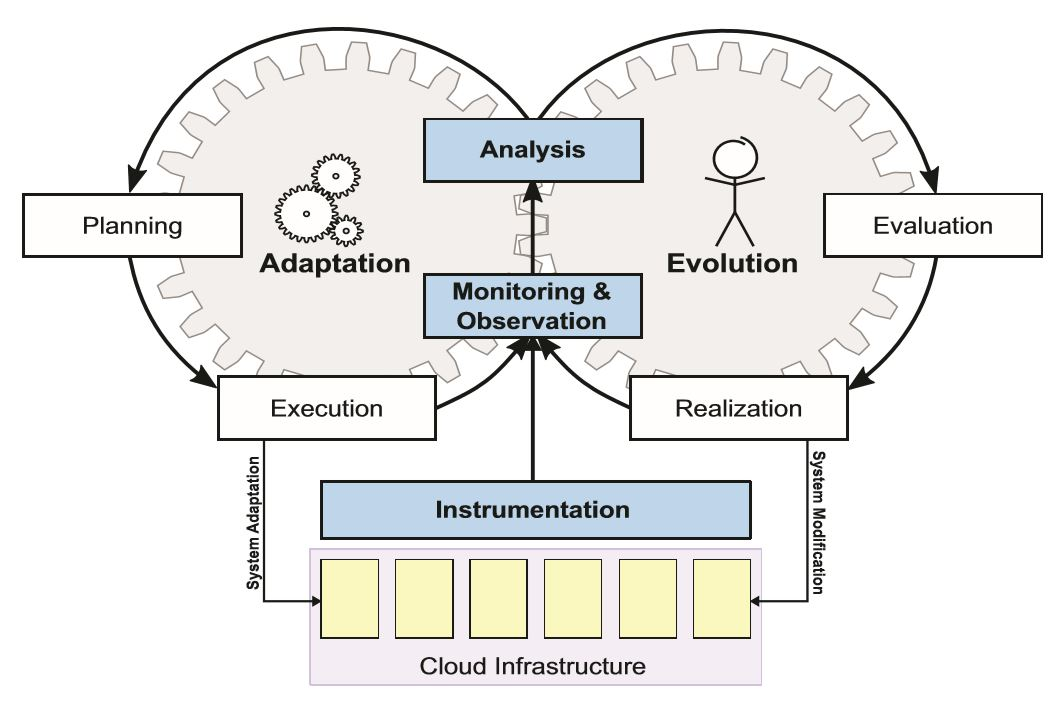
\includegraphics[width=0.65\textwidth]{pictures/iObserve_principle}
	\caption{iObserve cloud application life cycle \cite{Heinrich.2016b}}
	\label{fig:intro:iObserve}
\end{figure}

Currently, iObserve goes as far as updating the model. iObserve uses the TeeTime framework \cite{teetime.16.05.2017}, a pipeline-filter-framework with signal based stage invocation. More details on iObserve can be found in \cite{Heinrich.2016b}\cite{Heinrich.2016}.

\section{PerOpertyx}
\label{sec:Foundations:peropteryx}

"PerOpteryx is an optimization framework to improve component-based software architecture"\cite{PerOpteryx.b}. The optimization uses model-based quality prediction techniques. Starting from an input model, the framework generates multiple pareto optimal alternative deployments, based on given simulation and alternation algorithms. This approach is usually described as \textit{Design Space Exploration} (DSE). PerOpteryx uses multiple dimensions for its DSE, like alternating component multiplicities, runtime parameters or changing component allocations. The pareto optimal models are calculated through multiple iterations of a series of tasks. Initially a variance of candidates is created through an evolutionary algorithm and random generation. In the next step, the candidates are analysed for the desired quality marks along the different dimensions. The iteration concludes with the elimination of poorly performing candidates. PerOpteryx is designed to optimize Palladio Component Models, is based on the \textit{Rich Client Platfrom} and uses the \textit{Opt4J Framework} \cite{Martens.2010}.


